\documentclass[11pt]{article}
\usepackage[a4paper,margin=1in]{geometry}
\usepackage{amsmath,amssymb,amsthm,mathtools}
\usepackage{graphicx,booktabs,longtable,array,enumitem,hyperref,xcolor,microtype}
\setlength{\emergencystretch}{2em}
\hypersetup{colorlinks=true,linkcolor=black,citecolor=blue!50!black,urlcolor=blue!50!black}
\newtheorem{definition}{Definition}
\newtheorem{proposition}{Proposition}
\newtheorem{lemma}{Lemma}
\newtheorem{corollary}{Corollary}
\newcommand{\Tr}{\operatorname{Tr}}
\newcommand{\End}{\operatorname{End}}
\newcommand{\Aprim}{\mathcal A_{\rm prim}}
\newcommand{\Jocc}{\mathcal J_s}

\title{\textbf{Finite Source Signatures, Joint Incidence, and Representation Uniqueness}\\
\large Tau Core Technical Paper I (Series Paper II)}
\author{Jozsef Olcsak\\\small Independent researcher}
\date{Draft v0.2 --- Last revised: 29 August 2026}

\begin{document}
\maketitle
\begin{abstract}
We study a finite source-selection problem that precedes terminal physical
readouts.  A complete typed source signature consists of a finite-dimensional
unital \(C^*\)-algebra, a faithful source state, multiplication and involution
data, and distinguished role elements or completely positive maps.  The GNS
construction then gives a unique minimal cyclic realization up to the typed
unitary equivalences already declared in the source packet.

This positive theorem does not make terminal marginals sufficient.  Two
faithful bipartite states can share both marginals and differ in a joint
moment.  More strongly, four-qubit states can share every proper marginal
while differing along the 81-dimensional weight-four Pauli subspace; proper
marginals span only 174 of 255 traceless directions.  A single source-owned
onto joint incidence with positive stiffness is sufficient to generate a
faithful joint Gram state and hence all finite mixed moments.  Equivalently,
one coherent source homomorphism \(\Pi_{\rm phys}\) selects the physical
relation ideal and its faithful quotient representation.

We extend the four-qubit count to arbitrary \(n\)-partite qudit systems and
give singular-value bounds that quantify how an onto incidence becomes
ill-conditioned before rank is lost.  The results characterize sufficient
finite source information and exact non-identifiability boundaries.  They do
not prove that a physical base--seed parent creates, selects, or occupies the
required joint incidence or \(\Pi_{\rm phys}\), and they do not derive
terminal physics, the Standard Model, or empirical validation.
Later source-selection results sharpen this boundary: cyclic generated support
is sufficient to reach every typed source block, and occupied stable records
select the complete packet inside the declared source-irredundant MVP class.
Neither statement identifies that class with the unrestricted physical parent.
The common readout architecture further requires one source-owned observer
access map before terminal branching; separate terminal marginals do not
establish that shared morphology-conditioned origin.
This is the second stage of a seven-stage foundation programme: Paper I freezes
the architecture and conditional completion, Paper III analyzes record
transport, Paper IV isolates physical parent-law realization, Paper V develops
temporal descent and Paper VI the quantum terminal.  Paper VII is issued as the
focused VII-A--VII-C triptych.  These downstream papers do not alter the
source-signature theorems proved here or select their physical occupation.
\end{abstract}

\paragraph{Inherited morphology terminology.}
Following Foundation Paper I, $B_\tau^{\rm base}$ is the pre-readout
carrier/support context, the seed is its base-readable relational/loading
pattern, and $M_\tau^\star$ is the complete \emph{stabilized morphological
response configuration}; ``morphological body'' is shorthand.  Atemporal
selection of that configuration is distinct from literal traversal and from
observer time.  This paper reconstructs a declared source representation and
does not alter that ontology.
Under MRC-DEF2, parent-side ``objects'' are typed pregeometric relational
candidates, not ordinary bodies already embedded in recovered spacetime;
their Nature occupation remains open and ordinary objects occur downstream.
\begin{center}
\fbox{\begin{minipage}{.90\linewidth}\small
\textbf{Source-characteristic refinement inherited by this paper.}
A complete finite source signature must retain both the decoded seed and all
nonredundant base moduli:
\[
 \mathfrak c_{B,s}=(q_B,\beta_B).
\]
Only the connected fibers of this complete map are presentation redundancy.
Consequently a fixed-seed direction with $D\beta_B\ne0$ is physical source
information and may not be removed by the finite GNS or marginal quotient.
The representation theorems below apply to the resulting complete quotient;
they do not prove that the listed $\beta_B$ is exhaustive in Nature.
\end{minipage}}
\end{center}
\begin{center}
\fbox{\begin{minipage}{.90\linewidth}
\textbf{Dependency and ownership box.}

\textbf{Inputs from earlier papers:} Paper I supplies the types
\(s,M_\tau,A_O,T^{(a)},Q_O^{(a)}\), the body-first/source-freeze discipline and
the requirement of one common source before terminal branching.

\textbf{Results owned here:} complete finite typed source signatures; minimal
cyclic GNS uniqueness; exact marginal non-identifiability; onto-incidence
faithful occupation; representation/occupation separation; and the cyclic
generated-support criterion. Physical parent-class selection and record
transport are not proved here.  A downstream scalar-15/type-II application
uses this reconstruction language to identify one class-relative minimal
base--seed preimage; that specialization does not enlarge the theorem set of
this paper.
\end{minipage}}
\end{center}

\begin{center}
\fbox{\begin{minipage}{0.92\linewidth}\small
\textbf{Atemporal parent-realization terminology.}
Because the Tau parent is atemporal, phrases such as \emph{Nature selects} do
not denote an external agent or a later choice. Their precise meaning is the
internal physical implication
\[
 (B_\tau^{\rm phys},s_U,\mathcal L_{\rm parent})
 \Longrightarrow \mathfrak P,
\]
together with occupation of the support of the resulting packet
$\mathfrak P$. A theorem inside a declared completion proves only
class-relative realization. It does not prove this unrestricted base--seed
arrow, and agreement of finitely many terminal readouts cannot by itself
establish ambient-source exhaustivity. Current-facing statements therefore
use \emph{parent-law realization} and \emph{physical occupation}; any retained
legacy selection language is shorthand for this same distinction.
\end{minipage}}
\end{center}
\tableofcontents
\clearpage

\section{Problem and claim boundary}

\paragraph{Inherited observer co-descent convention.}
The symbol $O$ initially labels an occupied body-side carrier candidate,
not a detached or already operational observer.  Operational observerhood
requires a regular local rank-four Lorentzian descent, a stable
observer--source resolution map, and a nontrivial record/effect.  The observer
and its accessible four-dimensional world are therefore co-readouts of one
body-conditioned solution.  Neither a four-dimensional chart nor carrier
support alone is sufficient, and the readout relation is not an independent
physical layer.  This paper inherits that architecture from Paper I and
addresses only the finite source signature that can support it.

This finite signature does not by itself determine the upstream
four-dimensional reconstruction packet.  In particular, Paper II neither
selects a universal body-side derivation family $\mathfrak d_\tau$ nor its
source-owned observer restriction $R^{\mathfrak d}_{OS}$, and it does not
prove
\[
 \operatorname{rank}\!\left(\widetilde\Phi_{OS,x}
       \circ R^{\mathfrak d}_{OS}\right)=4.
\]
The same separator/representation data admit completions with different
visible restrictions, so rank four, Frobenius integrability,
Lorentz-conformal realizability and DA--ROOT/M4TR same-carrier agreement are
downstream physical gates.  Representation uniqueness in the declared finite
packet may constrain a candidate restriction only after that restriction is
source-owned; it cannot infer it from the desired terminal geometry.

\paragraph{Inherited minimal formation basis.}
Paper I defines the base as the protected zero-source response structure of a
frozen source-indexed body law, the universal seed as a response-distinct
base-relative source class, and the body as a stable selected nonneutral
response.  This split is canonical only after a physical zero source is fixed;
without it a common body-dependent refactorization makes base and seed
nonidentifiable.  Paper II takes this upstream formation datum as typed input.
Its finite-source uniqueness theorems do not construct the datum or select its
physical occupation.

The same scope boundary applies to temporal actuality.  A complete finite
signature may contain an occurrence-order covector, a positive response form
and the incidence data needed by a temporal completion.  Representation
uniqueness then says how that declared typed packet is realized; it does not
prove that the unrestricted base--seed source physically owns EOCC actuality,
that the body is literally traversed, or that observer time has been recovered.
The finite acyclic simultaneous-factor representation established downstream
also prevents interventional agreement from being used backward as a source-
signature selector.

\subsection{Joint representation--state compression of the separator data}

The common-source audit sharpens the finite-signature handoff.  Let
\begin{equation}
 \mathfrak J_*=(\Pi_*,\varphi_*),
 \qquad
 \Pi_*:\mathcal A_{\rm prim}^{\rm curr}
 \longrightarrow \mathcal A_{\rm post}(M_*)
 \label{eq:joint-source-datum}
\end{equation}
be a source-owned unital $*$-representation together with a state on its
retained central blocks.  Assume that the complete relation-defect functional
vanishes on $\Pi_*$, that the typed realization has one orbit after the
declared presentation/gauge quotient, that every retained central block is
irreducible up to its center, and that $\varphi_*$ is faithful on every such
block.  Then the apparently separate data are descendants of one object:
\begin{align}
 \mathcal J_{\rm phys}&=\ker\Pi_* ,&
 \mathcal J_{\rm mix}^{\rm phys}
   &=\ker\Pi_*\cap\mathcal A_{\rm mix},\nonumber\\
 \mathsf{Rep}^{\rm phys}_S&=\operatorname{Res}_S\Pi_* ,&
 \mathsf{Glue}_{34}^{\rm phys}
   &=\bigl(\operatorname{Res}_{P3}\Pi_*,
           \operatorname{Res}_{P4}\Pi_*\bigr),
 \label{eq:joint-source-descendants}\\
 p_{\rm occ}&=s(\varphi_*)=1
 &&\text{on every retained block}.\nonumber
\end{align}
Thus the mixed ideal, separator multiplicity matching, relative $P3$--$P4$
gluing and faithful occupation are not four independently adjustable source
switches.  They are jointly fixed, up to the declared typed gauge, once
$\mathfrak J_*$ is supplied.  In the minimum working completion the paired
separator-sign presentations are quotiented as one $\mathbb Z_2$ orbit; this
status must be reopened if a future source-frozen physical terminal is not
invariant under that action.

This is a compression theorem, not an unrestricted source theorem.  Equal
proper restrictions can carry different cross moments, and the current
narrow source admits equal-two-jet completions with different mixed words.
Consequently it does not entail $\mathfrak J_*$.  The enriched MVP adopts
Eq.~\eqref{eq:joint-source-datum} as one working completion, thereby closing
the subsidiary separator choices internally while leaving parent-law
realization, physical occupation and global terminal completeness open.

Suppose several terminal sectors have internally consistent local source
packets.  Their coexistence does not answer whether one physical source owns a
joint state, fixes all cross-sector relations, or selects one representation.
The finite question is
\begin{center}
\fbox{\begin{minipage}{.82\linewidth}
Which source data determine one minimal joint realization, and which
apparently complete data remain non-identifying?
\end{minipage}}
\end{center}

This paper proves conditional finite-algebra results.  It may claim
representation uniqueness after a complete source signature, exact marginal
no-go theorems, and an onto-incidence sufficient criterion.  It may not infer
physical occupation from these implications.  In particular, the notation
\(\Pi_{\rm phys}\) names a physical realization target; it does not assert that
the target has been derived.

\begin{figure}[t]
 \centering
 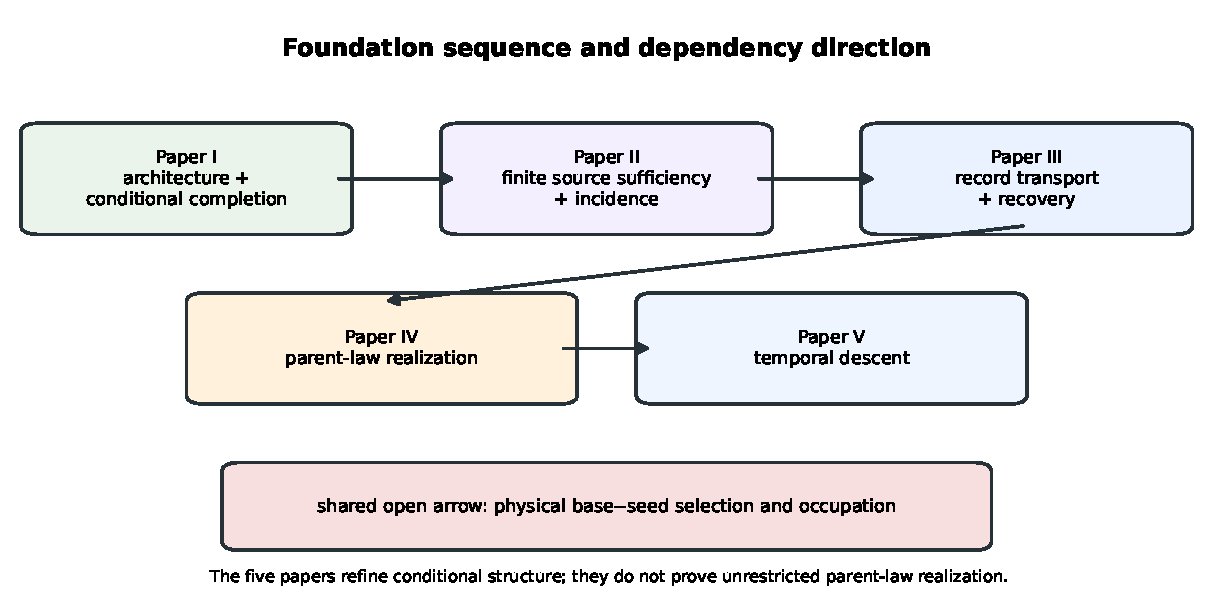
\includegraphics[width=.92\linewidth]{figures/fig_foundation_series_map.pdf}
 \caption{Dependency direction of the foundation sequence.  Paper II accepts
 the architectural types from Paper I and determines finite source
 sufficiency; it does not assume the transport conclusions of Paper III.}
 \label{fig:foundation-series-map}
\end{figure}

\paragraph{Series notation ledger.}
\begin{center}\small
\begin{tabular}{p{.16\linewidth}p{.53\linewidth}p{.20\linewidth}}
\toprule
Symbol & Series-wide meaning & Primary treatment\\
\midrule
\(s\) & source/seed packet prior to observer descent & Paper I\\
\(M_\tau\) & stabilized morphological response configuration (morphological body) & Paper I\\
\(\operatorname{Desc}_O\) & observer-indexed physical descent/readout & Paper I\\
\(\Pi_{\rm phys}\) & selected coherent source representation & Paper II\\
\(x_A\) & normalized finite source/body action separation & Papers I, III\\
\(x_Q\) & observer-carrier Uhlmann chord separation & Papers I, III\\
\(\mathcal C,\mathcal R\) & record map and recovery map & Paper III\\
\bottomrule
\end{tabular}
\end{center}

\subsection*{Morphology-conditioned readout interface}

Paper I writes every working primitive readout as
\begin{equation}
 \Xi_{OS}^{\rm cont}=\Phi_{OS}[M_\tau],
 \qquad
 D_{OS}^{\rm op}=Q_{OS,\delta}(\Xi_{OS}^{\rm cont}),
 \qquad
 Y_O^{(a)}=Q_O^{(a)}\circ T^{(a)}\circ A_O[M_\tau].
 \label{eq:mcpr-interface}
\end{equation}
For this paper, Eq.~\eqref{eq:mcpr-interface} is a source-signature
requirement. A complete joint packet must determine the common observer
access $A_O$, the typed terminal precursors $T^{(a)}$, the stable
resolution maps $Q_O^{(a)}$, and the overlap/null relations needed to compare
observers. Supplying separate terminal states without this common factor does
not prove common source ownership.

Before the finite quantizers act, the stacked terminal differential satisfies
\begin{equation}
 \operatorname{rank}
 \begin{bmatrix}
 D(T^{(1)}\circ A_O)\\[-1mm]
 \vdots\\[-1mm]
 D(T^{(n)}\circ A_O)
 \end{bmatrix}
 \leq \operatorname{rank}A_O.
 \label{eq:mcpr-rank}
\end{equation}
Consequently named time, quantum, gravity, matter, radiation or gauge
marginals can double count one accessible source direction. The GNS and joint
incidence results below decide representation only after the complete typed
signature is supplied; they do not derive $A_O$, the terminal family or its
physical occupation.

Paper I's exact migration criterion also fixes how a legacy source descriptor
may be imported here.  A historical map (L) is a descendant of the common
continuous descriptor precisely when
\begin{equation}
 L=U\circ\Xi_{OS}^{\rm cont},
 \qquad
 \Xi_{OS}^{\rm cont}(x)=\Xi_{OS}^{\rm cont}(x')
 \Longrightarrow L(x)=L(x').
 \label{eq:source-signature-migration}
\end{equation}
On a regular smooth branch this requires
$\ker D\Xi_{OS}^{\rm cont}\subseteq\ker DL$; equality gives the same local
quotient. Equal rank is insufficient, as shown by
$\Xi(x,y)=x$, $L(x,y)=x+y$. This paper may therefore reconstruct a legacy
finite packet only after this fibre test. It does not derive the physical
$Q_{OS,\delta}$, its cells, terminal calibration, $q_R(R)$, or Nature
occupation.

\begin{figure}[t]
 \centering
 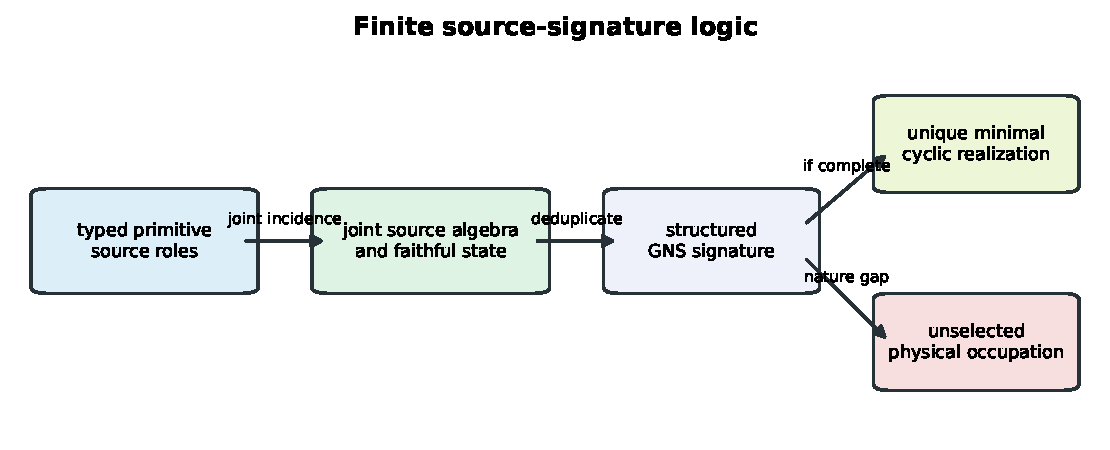
\includegraphics[width=.94\linewidth]{figures/fig_source_signature_pipeline.pdf}
 \caption{The finite logic.  Complete source data determine a minimal cyclic
 realization, but the physical base--seed law has not yet been shown to create
 or occupy those data.}
 \label{fig:signature-pipeline}
\end{figure}

\section{Finite typed source signatures}

Let \(\mathcal A_s\) be a finite-dimensional unital \(C^*\)-algebra.  After
the declared source-null quotient, assume a positive stiffness \(K_*>0\) and
a deduplicated source incidence \(R_s^{\rm dedup}\).  On its occupied ideal,
define
\begin{equation}
 G_s=R_s^{\rm dedup}K_*^{-1}(R_s^{\rm dedup})^\dagger,
 \qquad
 \rho_s={G_s\over\Tr G_s},
 \qquad
 \omega_s(a)=\Tr(\rho_sa).
 \label{eq:finite-source-state}
\end{equation}
If the incidence is onto the ideal, \(G_s>0\) and \(\omega_s\) is faithful
there.

Choose a source-orthonormal basis \(e_1,\ldots,e_d\).  Let
\(\mathbf z_s\) be the finite list of distinguished typed role elements and
CP maps retained by the claim.

\begin{definition}[Complete finite typed signature]
The source signature is
\begin{equation}
 \Sigma_s=
 \left(c_{ab}{}^c,j_a{}^b,\omega_s(e_a),
 [z_\alpha]_a,[\mathcal I_\beta]_{ab}\right),
 \quad
 e_ae_b=c_{ab}{}^ce_c,
 \quad e_a^*=j_a{}^be_b.
 \label{eq:signature}
\end{equation}
It is \emph{complete relative to a claim} when it contains the full abstract
algebra, faithful state and every typed element or map used by that claim.
Simultaneous source-basis changes are quotiented only when declared typed
source isometries.  Undeclared algebra automorphisms are not automatically
physical equivalences.
\end{definition}

This is finite information: multiplication, involution, state and role arrays.
Completeness is claim-relative, not a statement that all parent information is
accessible.

Every finite-dimensional unital \(C^*\)-algebra has a decomposition
\begin{equation}
 \mathcal A_s\cong\bigoplus_{\alpha=1}^{r}M_{n_\alpha}(\mathbb C).
 \label{eq:wedderburn}
\end{equation}
The signature must therefore record not only dimensions but the multiplication
and involution that distinguish the blocks and their typed roles.  A faithful
state has strictly positive density on every occupied central block.  Dropping
a zero-weight block is an occupation decision; it is not a consequence of GNS
uniqueness on the remaining support.

\subsection{Four logically distinct questions}

The following distinctions are used throughout.
\begin{longtable}{p{.18\linewidth}p{.35\linewidth}p{.36\linewidth}}
\toprule
Question & Mathematical content & What can answer it here?\\
\midrule
\endhead
Existence & Does at least one realization of the typed packet exist? & An
explicit representation or incidence construction.\\
Uniqueness & Are all minimal cyclic realizations of the same complete packet
typed-unitarily equivalent? & The finite GNS theorem below.\\
Identifiability & Do the retained observables determine the complete packet? &
A separating-rank test, or a countermodel in the kernel of the retained
descriptor.\\
Physical realization & Why does the base--seed parent law realize and occupy
one admissible packet? & A
base--seed source law or independent experiment; neither follows from the
other three rows.\\
\bottomrule
\end{longtable}

In particular, uniqueness conditional on \(\Sigma_s\) cannot repair an
incomplete descriptor.  Conversely, an informationally complete descriptor
does not prove physical occupation of its reconstructed point.

\begin{definition}[Typed equivalence]
Two realizations are equivalent only if a unitary intertwines the represented
algebra, maps the cyclic source vector, preserves the declared central blocks,
and intertwines every distinguished role element and source map.  Automorphisms
not included in this equivalence group remain physically distinguishable data.
\end{definition}

\section{GNS representation uniqueness}

\begin{proposition}[Finite source-signature representation uniqueness]
Fix \((\mathcal A_s,\omega_s,\mathbf z_s)\) through one complete signature
\(\Sigma_s\), with \(\omega_s\) faithful.  Any two minimal cyclic finite
realizations of these data are related by a unique unitary that maps one cyclic
vector to the other, implements the fixed algebra identification, and
intertwines every distinguished element and the represented action of every
distinguished linear or completely positive source map.
\end{proposition}
\begin{proof}
Faithfulness gives
\(\mathcal N_{\omega_s}=\{a:\omega_s(a^*a)=0\}=\{0\}\).  The GNS Hilbert space
is the completion of \(\mathcal A_s\) under
\(\langle a,b\rangle_s=\omega_s(a^*b)\), with cyclic vector \([1]\) and left
representation \(\pi_s(a)[b]=[ab]\).  For two minimal cyclic realizations set
\begin{equation}
 U\pi_1(a)\Omega_1=\pi_2(a)\Omega_2.
\end{equation}
Equality of \(\omega_s\) makes \(U\) isometric; cyclic minimality makes its
range dense, hence unitary.  For a distinguished source map
\(\mathcal I_\beta:\mathcal A_s\to\mathcal A_s\), define on the cyclic
domain
\begin{equation}
 \widehat{\mathcal I}_{\beta,i}\,\pi_i(a)\Omega_i
 =\pi_i(\mathcal I_\beta(a))\Omega_i.
 \label{eq:represented-source-map}
\end{equation}
In finite dimension this is a bounded linear operator whenever the displayed
rule is well defined on the GNS quotient; faithfulness makes that quotient
trivial here.  The definition of \(U\) gives
\(U\widehat{\mathcal I}_{\beta,1}
=\widehat{\mathcal I}_{\beta,2}U\) on the cyclic span.  The same calculation
handles represented role elements.  The cyclic span fixes \(U\) uniquely.
This is the
finite GNS uniqueness mechanism \cite{Segal1947}.
\end{proof}

Complete positivity is not used to prove unitary uniqueness; it records the
physical type of an admissible source operation.  Stinespring dilation gives a
standard representation of such maps, but the dilation environment is not
unique without its own minimality condition \cite{Stinespring1955}.  The
present theorem therefore claims uniqueness of the typed minimal cyclic
realization, not uniqueness of every implementation of its CP operations.

The theorem begins \emph{after} the source signature has been supplied.  It
does not show that the unrestricted physical parent law realizes and occupies
\(\Sigma_s\).  If a signature map
\(\Phi_s\) is faithful modulo typed source isometry and the post-quotient
metric is positive, then
\begin{equation}
 \mathcal D_s(C)=\lVert\Phi_s(C)-\Sigma_s\rVert^2
 \label{eq:signature-defect}
\end{equation}
has at most one zero completion class.  Existence of an occupied zero remains
an independent physical requirement.

\section{Marginals do not select a joint source}

\begin{proposition}[Two-sector marginal no-go]
Complete faithful source states on separate sectors do not generally determine
their joint source state.
\end{proposition}
\begin{proof}
For two qubits, compare
\begin{equation}
 \rho_0={I_4\over4},\qquad
 \rho_\epsilon={1\over4}
 \left(I_4+\epsilon\,\sigma_z\otimes\sigma_z\right),
 \qquad0<|\epsilon|<1.
 \label{eq:bipartite-countermodel}
\end{equation}
Both states are faithful and both marginals equal \(I_2/2\).  Their joint
\(\sigma_z\otimes\sigma_z\) moments are respectively zero and \(\epsilon\).
\end{proof}

Thus compatible gravity, clock, radiation, quantum, matter or gauge marginals
cannot be promoted to one joint physical source merely by being placed side by
side.  Cross-sector moments spanning the missing self-adjoint source
directions are required.

\section{All proper marginals remain incomplete}

For four qubits the traceless Pauli words have total dimension
\(4^4-1=255\).  Words of weights one, two and three contribute
\begin{equation}
 {4\choose1}3+{4\choose2}3^2+{4\choose3}3^3
 =12+54+108=174.
 \label{eq:proper-span}
\end{equation}
The remaining weight-four subspace has dimension \(3^4=81\).

\begin{figure}[t]
 \centering
 
\includegraphics[width=.86\linewidth]{figures/fig_pauli_dimension_audit.pdf}
 \caption{Exact Pauli-word dimension audit.  Every proper marginal can access
 weights at most three; the 81 weight-four directions remain invisible.}
 \label{fig:pauli-audit}
\end{figure}

\begin{proposition}[Four-sector all-proper-marginal no-go]
There are faithful four-qubit states with identical marginals on every proper
subsystem and different genuine four-sector moments.
\end{proposition}
\begin{proof}
Let
\begin{equation}
 \rho_\epsilon={1\over16}
 \left(I_{16}+\epsilon\,\sigma_z^{\otimes4}\right),
 \qquad0<|\epsilon|<1.
 \label{eq:four-sector-family}
\end{equation}
Its eigenvalues are \((1\pm\epsilon)/16>0\).  Tracing out any nonempty factor
annihilates the Pauli product because \(\Tr\sigma_z=0\), so every proper
marginal is maximally mixed and independent of \(\epsilon\).  Yet
\(\Tr(\rho_\epsilon\sigma_z^{\otimes4})=\epsilon\).
\end{proof}

The number 81 belongs specifically to this four-qubit Pauli decomposition.
It is not a representation-independent count for every four-sector model.
The invariant lesson is that all proper marginals may leave genuine joint
directions unresolved.

\subsection{General \(n\)-partite qudit count}

The preceding example is the smallest calculation used by the Tau packet, but
the obstruction is general.  Fix a Hilbert--Schmidt orthogonal Hermitian basis
\(\{I,T_1,\ldots,T_{d^2-1}\}\) on one qudit, with every \(T_a\) traceless.
The tensor words of weight \(w\) have dimension
\begin{equation}
 N_w={n\choose w}(d^2-1)^w.
 \label{eq:weight-count}
\end{equation}

\begin{proposition}[All-proper-marginal kernel for \(n\) qudits]
For \(n\ge2\), the linear descriptor consisting of every proper marginal
annihilates the full-weight tensor subspace of dimension
\((d^2-1)^n\).  Hence the descriptor rank on traceless Hermitian operators is
at most
\begin{equation}
 \sum_{w=1}^{n-1}{n\choose w}(d^2-1)^w
 =d^{2n}-1-(d^2-1)^n.
 \label{eq:proper-marginal-rank}
\end{equation}
There are faithful density operators with identical proper marginals and
different full-weight moments.
\end{proposition}
\begin{proof}
Tracing out any factor of a full-weight word
\(T_{a_1}\otimes\cdots\otimes T_{a_n}\) gives zero because each local factor
is traceless.  Linear independence of the tensor-product basis gives the
kernel dimension.  For any nonzero Hermitian full-weight word \(X\), set
\begin{equation}
 \rho_\epsilon={I\over d^n}+\epsilon X,
 \qquad
 |\epsilon|<{1\over d^n\lVert X\rVert_{\rm op}}.
 \label{eq:general-marginal-family}
\end{equation}
Then \(\rho_\epsilon>0\), has unit trace, and every proper marginal is
independent of \(\epsilon\), while \(\Tr(\rho_\epsilon X)\) varies linearly.
\end{proof}

For \(n=4,d=2\), Eq.~\eqref{eq:proper-marginal-rank} returns
\(255-81=174\).  The theorem is an identifiability statement, not a claim that
physical source sectors are qudits.  It formalizes why assembling all lower
order readouts need not determine their common parent relation, a familiar
form of the quantum marginal problem \cite{Klyachko2006,Bravyi2004,
LindenPopescuWootters2002}.

\subsection{Descriptor rank criterion}

Let \(V_J\) be the real vector space of traceless self-adjoint operators on a
declared joint carrier, and let
\(D:V_J\to\mathbb R^m\) collect all retained expectation values.  The joint
state is locally identifiable from those linear data exactly when
\begin{equation}
 \ker D=\{0\}.
 \label{eq:descriptor-rank}
\end{equation}
If \(\ker D\ne\{0\}\), any sufficiently small Hermitian perturbation along a
kernel direction preserves positivity around a faithful state and produces a
locally indistinguishable state.  This turns ``descriptor completeness'' into
a finite rank test rather than a verbal completeness claim.

\begin{proposition}[Noise-stable linear identifiability]
Equip \(V_J\) and \(\mathbb R^m\) with fixed Euclidean norms and let
\(\sigma_D>0\) be the smallest singular value of an injective descriptor
\(D\).  If two states satisfy
\begin{equation}
 \lVert D(\rho-\sigma)\rVert\le\delta,
 \label{eq:noisy-descriptor}
\end{equation}
then
\begin{equation}
 \lVert\rho-\sigma\rVert\le{\delta\over\sigma_D}.
 \label{eq:descriptor-stability}
\end{equation}
If \(D\) is not injective, no finite bound of this form can control components
in \(\ker D\).
\end{proposition}
\begin{proof}
By the singular-value variational definition,
\(\lVert DX\rVert\ge\sigma_D\lVert X\rVert\) for all \(X\in V_J\).
Apply this to \(X=\rho-\sigma\).  If \(X\in\ker D\setminus\{0\}\), the
descriptor difference vanishes while \(\lVert X\rVert\) does not.
\end{proof}

The bound depends on the declared normalization of observables and noise.  It
is not invariant under arbitrary rescaling of descriptor rows, so a physical
audit must freeze those units before reporting \(\sigma_D\).  Statistical
confidence regions may then be propagated through the same singular-value
decomposition; they do not change the exact kernel.

For orientation, three qubits have \(4^3-1=63\) traceless Pauli directions.
All one- and two-body words span
\begin{equation}
 {3\choose1}3+{3\choose2}3^2=9+27=36,
\end{equation}
leaving 27 weight-three directions invisible to every proper marginal.  Four
qubits enlarge these numbers to 174 visible and 81 invisible directions.  The
growth is structural: adding more lower-order precision does not reveal an
exact full-weight kernel direction.

\section{One onto joint incidence is sufficient}

The positive replacement is not an independently fitted coefficient for every
missing word.

\begin{proposition}[Onto-incidence faithful-state theorem]
Let \(\mathcal H_J\) be an occupied finite joint carrier, let
\(\mathcal E_J\) be the source-leg Hilbert space, let
\(K_s\in\End(\mathcal E_J)\) be positive definite, and let
\(R_J:\mathcal E_J\to\mathcal H_J\) be a source-owned onto incidence.  Then
\begin{equation}
 G_J=R_JK_s^{-1}R_J^\dagger,
 \qquad
 \rho_J={G_J\over\Tr G_J}
 \label{eq:joint-gram-state}
\end{equation}
defines a faithful density operator on \(\mathcal H_J\).  Once the typed joint
role algebra is represented on \(\mathcal H_J\), it fixes every finite mixed
moment of that representation.
\end{proposition}
\begin{proof}
Surjectivity of \(R_J\) makes \(R_J^\dagger\) injective.  For nonzero
\(v\in\mathcal H_J\),
\begin{equation}
 \langle v,G_Jv\rangle
 =\langle R_J^\dagger v,K_s^{-1}R_J^\dagger v\rangle>0.
\end{equation}
Hence \(G_J>0\), the normalized state is faithful, and linearity assigns all
mixed-word expectations.
\end{proof}

Onto incidence is sufficient, not necessary in every possible presentation.
It is also not selected by the separate sector marginals.

\subsection{Quantitative stability before rank loss}

Surjectivity is a sharp condition, but experiments and numerical source
reconstructions require a condition number.  Write
\(k_{\min}=\lambda_{\min}(K_s)\),
\(k_{\max}=\lambda_{\max}(K_s)\), and let
\(\sigma_{\min}(R_J)\), \(\sigma_{\max}(R_J)\) be the extremal singular values
on the non-null source quotient.

\begin{proposition}[Joint-Gram eigenvalue bounds]
If \(R_J\) is onto, then
\begin{equation}
 {\sigma_{\min}(R_J)^2\over k_{\max}}
 \le \lambda_{\min}(G_J)
 \le \lambda_{\max}(G_J)
 \le {\sigma_{\max}(R_J)^2\over k_{\min}}.
 \label{eq:gram-bounds}
\end{equation}
Consequently,
\begin{equation}
 \kappa(G_J)\le
 \kappa(K_s)\left({\sigma_{\max}(R_J)\over
 \sigma_{\min}(R_J)}\right)^2.
 \label{eq:gram-condition}
\end{equation}
\end{proposition}
\begin{proof}
For unit \(v\in\mathcal H_J\),
\begin{equation}
 {\lVert R_J^\dagger v\rVert^2\over k_{\max}}
 \le \langle v,G_Jv\rangle
 \le {\lVert R_J^\dagger v\rVert^2\over k_{\min}}.
\end{equation}
The min--max principle and the singular values of \(R_J^\dagger\) give
Eq.~\eqref{eq:gram-bounds}; division gives
Eq.~\eqref{eq:gram-condition}.
\end{proof}

Thus the exact theorem has an observable precursor: as
\(\sigma_{\min}(R_J)\to0\), the reconstructed joint state becomes poorly
conditioned before faithfulness is lost.  A small singular value is not new
physics by itself; it may also signal an incomplete descriptor, calibration
degeneracy, or insufficient data.  If \(R_J\) is not onto, then
\begin{equation}
 \ker G_J=\ker R_J^\dagger=(\operatorname{ran}R_J)^\perp.
 \label{eq:gram-kernel}
\end{equation}
The unresolved directions are therefore explicit rather than absorbed into a
fitted terminal correction.

\section{The coherent physical source map}

Let the once-owned primitive roles generate a universal typed unital
\(*\)-algebra \(\Aprim\) modulo relations already fixed source-side.  One
source-owned unital \(*\)-homomorphism
\begin{equation}
 \Pi_{\rm phys}:\Aprim\longrightarrow\mathcal B(\mathcal H_{\rm post})
 \label{eq:pi-phys}
\end{equation}
selects the physical relation ideal \(\ker\Pi_{\rm phys}\) and a faithful
representation of the quotient
\(\Aprim/\ker\Pi_{\rm phys}\).

\begin{proposition}[Compression of finite joint selection]
Once the primitive typed presentation is fixed, selection of the joint ideal,
quotient representation and distinguished role images can be compressed to
one coherent \(\Pi_{\rm phys}\), rather than a table of independently fitted
cross-terminal gains.
\end{proposition}
\begin{proof}
The kernel of a unital \(*\)-homomorphism is a two-sided \(*\)-ideal.  The
first isomorphism theorem identifies the quotient with its image.  The images
of the typed generators then determine the represented role packet and all
algebraically generated mixed relations.
\end{proof}

The proposition does not construct or occupy \(\Pi_{\rm phys}\).  Distinct
homomorphisms can preserve all currently fixed marginal and overlap data while
changing mixed moments.  A complete seed-owned relation presentation and a
unique typed-unitary zero orbit would be sufficient, but are not derived here.

\subsection{What \(\Pi_{\rm phys}\) does and does not select}

The homomorphism fixes algebraic relations and a represented quotient.  It does
not by itself fix a faithful state on that quotient.  Conversely, the
incidence/stiffness pair in Eq.~\eqref{eq:joint-gram-state} fixes a density
operator only after the carrier and represented role algebra are known.  The
two data are complementary:
\begin{equation}
 \Pi_{\rm phys}:
 \text{relations and representation},
 \qquad
 (R_J,K_s):
 \text{occupation and joint state}.
 \label{eq:representation-state-split}
\end{equation}
Calling them ``equivalent'' would require an additional common-source theorem
that reconstructs each from the other.  No such theorem is assumed here.

\begin{proposition}[Faithful quotient representation]
If \(\Pi_{\rm phys}:\Aprim\to\mathcal B(\mathcal H_{\rm post})\) is a unital
\(*\)-homomorphism, then the induced map
\begin{equation}
 \widetilde\Pi_{\rm phys}:
 \Aprim/\ker\Pi_{\rm phys}\longrightarrow
 \operatorname{im}\Pi_{\rm phys}
 \label{eq:faithful-quotient-map}
\end{equation}
is a faithful unital \(*\)-isomorphism.
\end{proposition}
\begin{proof}
The kernel is a two-sided closed \(*\)-ideal.  The first isomorphism theorem
makes the induced map bijective and \(*\)-preserving; injectivity is precisely
faithfulness on the quotient.
\end{proof}

The choice of \(\ker\Pi_{\rm phys}\) remains physical information.  The same
primitive generator list can admit inequivalent ideals and hence inequivalent
joint physics.  Marginal agreement cannot select among them when the
distinguishing relation lies in the marginal descriptor kernel.

\section{Countermodels separating the logical levels}

The preceding results are easiest to audit through finite controls.

\paragraph{Same marginals, different state.}
Equation~\eqref{eq:bipartite-countermodel} keeps both reduced density matrices
fixed while changing one joint moment.  Identifiability fails even though both
joint states exist.

\paragraph{Same presentation, different quotient.}
Let \(\Aprim=\mathbb C[x]/(x^2-x)\), viewed as a unital \(*\)-algebra with
\(x=x^*\).  The characters \(\Pi_0(x)=0\) and \(\Pi_1(x)=1\) are both unital
\(*\)-homomorphisms but have different kernels.  A generator name and its
typing therefore do not select one physical relation ideal.

\paragraph{Same carrier dimension, different incidence rank.}
Take \(K_s=I_2\), \(R_{\rm onto}=I_2\), and
\begin{equation}
 R_{\rm deficient}=\begin{pmatrix}1&0\\0&0\end{pmatrix}.
\end{equation}
The first produces \(G_J=I_2\); the second produces a rank-one Gram operator.
Carrier dimension alone therefore does not imply faithful occupation.

\paragraph{Near-singular but onto incidence.}
For \(R_\delta=\operatorname{diag}(1,\delta)\), \(0<\delta\ll1\), the joint
state is faithful but \(\kappa(G_J)=\delta^{-2}\).  Exact identifiability can
coexist with severe practical instability, which is why the singular-value
ledger is part of the operational audit.

\section{Worked end-to-end finite packet}

We now run one packet from typed source data to represented mixed moments.  It
is deliberately elementary: its purpose is to expose every domain, rank and
normalization used by the abstract theorems, not to model a physical Tau
carrier.

Let the joint carrier and source-leg spaces both be \(\mathbb C^2\), and set
\begin{equation}
 K_s=\begin{pmatrix}k_0&0\\0&k_1\end{pmatrix},
 \qquad
 R_\delta=\begin{pmatrix}1&0\\0&\delta\end{pmatrix},
 \qquad k_0,k_1>0,\quad\delta>0.
 \label{eq:worked-source-data}
\end{equation}
The represented role algebra is \(\mathcal A_s=M_2(\mathbb C)\), with typed
Hermitian generators \(I,X,Y,Z\) and Hilbert--Schmidt reference pairing
\(\langle a,b\rangle_{\rm HS}=\Tr(a^\dagger b)\).  The occupied faithful
state will be generated by the incidence.  Its Gram operator is
\begin{equation}
 G_\delta=R_\delta K_s^{-1}R_\delta^\dagger
 =\begin{pmatrix}k_0^{-1}&0\\0&\delta^2k_1^{-1}\end{pmatrix},
 \label{eq:worked-gram}
\end{equation}
and therefore
\begin{equation}
 \rho_\delta=
 {1\over k_0^{-1}+\delta^2k_1^{-1}}
 \begin{pmatrix}k_0^{-1}&0\\0&\delta^2k_1^{-1}\end{pmatrix}.
 \label{eq:worked-state}
\end{equation}

For every \(\delta>0\), \(R_\delta\) is onto and \(\rho_\delta\) is faithful.
At \(\delta=0\), the second carrier direction lies in
\(\ker R_0^\dagger\), \(G_0\) has rank one, and the full-carrier faithful-state
claim fails exactly as Eq.~\eqref{eq:gram-kernel} predicts.  With \(k_0=k_1=1\),
\begin{equation}
 \lambda_{\min}(G_\delta)=\delta^2,
 \qquad
 \lambda_{\max}(G_\delta)=1,
 \qquad
 \kappa(G_\delta)=\delta^{-2}
 \quad(0<\delta\le1).
 \label{eq:worked-conditioning}
\end{equation}

The full Bloch descriptor
\begin{equation}
 D_{XYZ}(\rho)=
 \bigl(\Tr\rho X,\Tr\rho Y,\Tr\rho Z\bigr)
 \label{eq:bloch-descriptor}
\end{equation}
is injective on trace-one Hermitian matrices and reconstructs
\begin{equation}
 \rho={1\over2}\bigl(I+D_X X+D_Y Y+D_Z Z\bigr).
 \label{eq:bloch-reconstruction}
\end{equation}
For Eq.~\eqref{eq:worked-state}, \(D_X=D_Y=0\) and
\begin{equation}
 D_Z={k_0^{-1}-\delta^2k_1^{-1}
 \over k_0^{-1}+\delta^2k_1^{-1}}.
 \label{eq:worked-bloch-z}
\end{equation}
Keeping only \(D_Z\) would identify this diagonal family after that family was
frozen, but would not identify an arbitrary qubit state: the \(X\) and \(Y\)
directions would remain in the descriptor kernel.

Finally take \(\Aprim=M_2(\mathbb C)\) with its Pauli presentation and choose
\begin{equation}
 \Pi_{\rm phys}=\operatorname{id}_{M_2}:\Aprim\to\mathcal B(\mathbb C^2).
 \label{eq:worked-pi}
\end{equation}
This is a unital \(*\)-homomorphism with zero kernel, so it supplies the
faithful quotient representation.  The dephasing map
\(a\mapsto P_0aP_0+P_1aP_1\) is unital and completely positive but not
multiplicative on \(M_2\); it cannot replace \(\Pi_{\rm phys}\) in the quotient
theorem even though it preserves the diagonal family.

\begin{figure}[t]
 \centering
 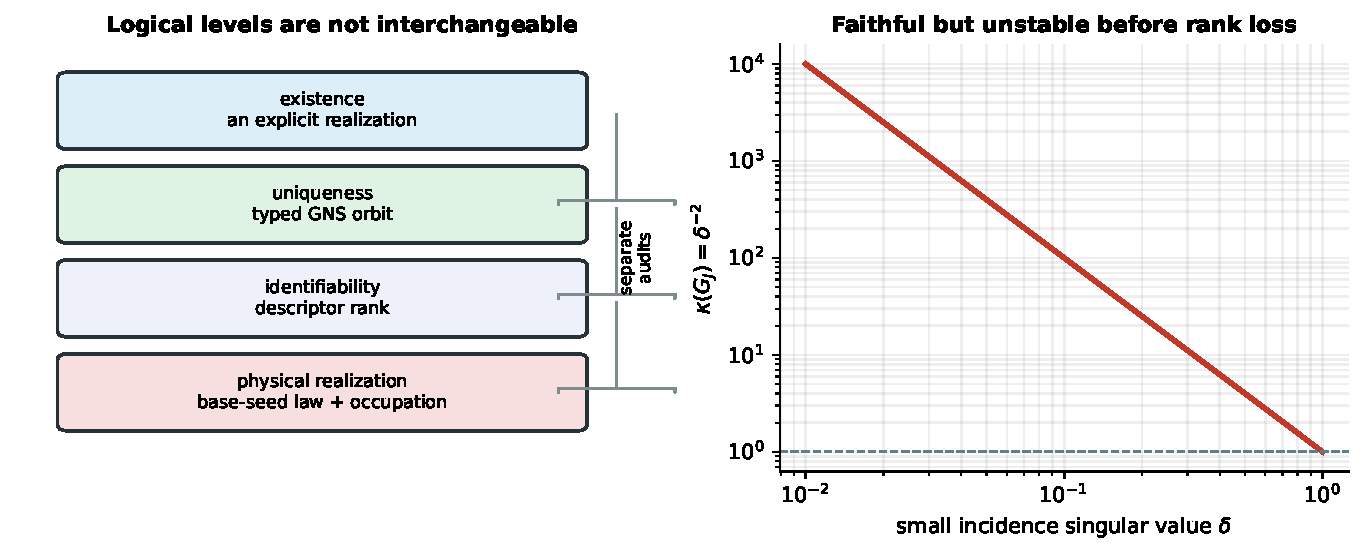
\includegraphics[width=.96\linewidth]{figures/fig_selection_stability.pdf}
 \caption{Left: existence, uniqueness, identifiability and physical realization
 require separate audits.  Right: the worked packet stays faithful for every
 \(\delta>0\) while its Gram condition number diverges as rank loss is
 approached.}
 \label{fig:selection-stability}
\end{figure}

The complete finite certificate for this toy is therefore
\begin{equation}
 \mathfrak C_\delta=
 \left(M_2,\omega_\delta,K_s,R_\delta,D_{XYZ},
 \Pi_{\rm phys}=\operatorname{id},
 \mathcal G_{\rm eq}=\{I\},
 \mathsf{occupation}=\rho_\delta\right).
 \label{eq:worked-certificate}
\end{equation}
where \(\omega_\delta(a)=\Tr(\rho_\delta a)\).  It proves internal existence,
typed GNS uniqueness, descriptor
identifiability, onto-incidence faithfulness and representation consistency.
It does \emph{not} prove that a base--seed parent selects any member of this
family, any value of \(k_0,k_1,\delta\), or the identity representation as a
physical law.

\subsection{Failure matrix for the worked packet}

The same example separates failures that would otherwise look alike in an
endpoint fit.
\begin{longtable}{p{.22\linewidth}p{.28\linewidth}p{.38\linewidth}}
\toprule
Modification & Mathematical result & Scientific diagnosis\\
\midrule
\endhead
\(k_0=k_1\), \(\delta=1\) & \(G=I\),
\(\rho=I/2\), \(\kappa(G)=1\) & Symmetric, well-conditioned occupied packet;
still no proof of physical realization.\\
\(0<\delta\ll1\) & \(G>0\) but
\(\kappa(G)=\delta^{-2}\gg1\) & Exact faithfulness survives, while finite
precision makes the weak direction difficult to reconstruct.\\
\(\delta=0\) & \(R\) is not onto and \(G\) has rank one & The claimed
full-carrier faithful occupation is false; support reduction must be declared.\\
Retain \(D_Z\) only & Diagonal states are separated, arbitrary qubit states
are not & The descriptor is complete only relative to a frozen commuting
family; off-diagonal completion is unidentifiable.\\
Replace \(\Pi_{\rm phys}\) by dephasing & The map is unital CPTP but not a
\(*\)-homomorphism & It may define an irreversible record process, not the
relation-ideal quotient used in Proposition 8.\\
Fit \(k_0,k_1,\delta\) from the same terminal outcome & Many packets can
reproduce one diagonal state & Endpoint agreement cannot establish upstream
source ownership or select the physical parameter triple.\\
\bottomrule
\end{longtable}

The rows give mutually different remedies.  Rank loss requires a smaller
support theorem; descriptor failure requires additional predeclared
observables; nonmultiplicative dynamics require a CP/recovery analysis; and
failure of unrestricted parent-law realization requires an upstream source
law or independent
overdetermination.  None is repaired by merely improving the fit of
Eq.~\eqref{eq:worked-state} to one measured density matrix.

\section{Operational source-completeness audit}

A finite source-signature claim should declare:
\begin{enumerate}[label=(S\arabic*)]
 \item the source algebra and true-null quotient;
 \item the faithful state or the incidence/stiffness pair generating it;
 \item all typed primitive roles and ownership multiplicities;
 \item the cross-sector observables required by the claim;
 \item the equivalence group and every non-quotiented automorphism;
 \item the rank test showing that retained observables separate the joint
 self-adjoint algebra; and
 \item whether existence, uniqueness and physical occupation are each proved,
 assumed or open.
\end{enumerate}

Passing this audit proves informational completeness relative to the declared
finite claim.  It does not prove unrestricted parent-law realization or
physical occupation of the audited source.

\subsection{A reproducible finite audit matrix}

For a concrete model the declarations above reduce to finite linear algebra.
The following matrix separates calculations from physical assumptions.
\begin{longtable}{p{.27\linewidth}p{.32\linewidth}p{.31\linewidth}}
\toprule
Object & Reproducible check & Failure meaning\\
\midrule
Algebra packet & Verify associativity, unit and involution arrays in
Eq.~\eqref{eq:signature}. & The proposed typed source is not a
\(C^*\)-algebra presentation.\\
State packet & Diagonalize \(\rho_s\) on every declared occupied block. & A
zero eigenvalue requires support reduction or a nonfaithful theorem.\\
Descriptor & Compute \(\operatorname{rank}D\) on the declared self-adjoint
joint space. & Kernel directions are not identified by the retained data.\\
Incidence & Compute rank and singular values of \(R_J\) after true-null
quotient. & Rank loss forbids faithful Gram occupation; small singular values
signal instability.\\
Representation & Verify multiplicativity, unit and dagger preservation of
\(\Pi_{\rm phys}\). & A merely unital linear or CP map does not define the
claimed relation ideal by the first isomorphism theorem.\\
Equivalence & Test whether candidate solutions lie in the declared typed
unitary orbit. & An undeclared automorphism is a second physical completion,
not gauge by default.\\
Ownership & Trace every retained parameter to one source ledger entry. & A
terminally inserted cross-gain violates source freeze.\\
\bottomrule
\end{longtable}

The audit is deliberately compatible with negative results.  A rank-deficient
descriptor is not repaired by fitting its kernel directions to terminal data;
it is reported as non-identifying.  A non-onto incidence is not promoted by
renaming its support the full carrier.  A second zero orbit is not quotient
gauge unless the equivalence group was declared before inspecting it.

\section{Relation to established finite-dimensional results}

The mathematical ingredients are standard; the contribution is their typed
source-selection arrangement and explicit claim boundary.  GNS gives a
canonical cyclic representation after an algebra and state are fixed
\cite{Segal1947}.  Stinespring characterizes completely positive maps through
dilations, but does not select a physical source state or a unique
nonminimal environment \cite{Stinespring1955}.  Quantum marginal theory asks
whether reduced states are compatible with a common global state and when
they determine it \cite{Klyachko2006,Bravyi2004,
LindenPopescuWootters2002}.  The present all-proper-marginal count is a direct
tensor-basis kernel calculation within that broader problem.

What is specific to this program is the division of labor:
\begin{equation}
 \text{typed source signature}
 \longrightarrow
 \begin{cases}
  \text{minimal cyclic representation},\\
  \text{descriptor-rank audit},\\
  \text{incidence-generated occupation},\\
  \text{explicit parent-realization blocker}.
 \end{cases}
 \label{eq:division-of-labor}
\end{equation}
No novelty is claimed for GNS, Stinespring theory, or the marginal problem
themselves.  Nor does the finite analysis establish quantum gravity or the
Standard Model.  Its use is to prevent several terminal reconstructions from
being mistaken for one physically selected common source.

\section{What a physical source theorem must add}

The remaining theorem cannot be another representation theorem conditional on
the desired packet.  It must provide a parent law whose occupied solutions
jointly determine:
\begin{enumerate}[label=(P\arabic*)]
 \item the primitive typed algebra and its relation ideal;
 \item the carrier and the physical homomorphism \(\Pi_{\rm phys}\);
 \item the source-leg stiffness \(K_s\) and incidence \(R_J\);
 \item a faithful occupied state or a declared support reduction;
 \item the equivalence group, including which automorphisms are gauge; and
 \item the terminally relevant descriptors, their common observer-access
 factor, stable resolution maps and overlap laws without endpoint-dependent
 tuning.
\end{enumerate}
An action principle could supply such data only if its variables and symmetry
group are specified before variation and if its stationary orbit is unique up
to the declared equivalence.  A reconstruction from public terminal data can
support or reject the rank, positivity and shared-parameter consequences of a
candidate packet, but cannot by itself prove that the base--seed parent is its
ontological source.

This distinction gives a finite reopening rule.  The physical-realization branch
is promoted only by either (i) a source theorem deriving (P1)--(P6), or (ii) a
source-frozen experiment whose independent observables overdetermine the same
packet and reject its allowed alternatives.  Additional terminal fits without
such overdetermination do not close the arrow.

\subsection{Later source-completion status}

The primary source-irredundant enriched completion now conditionally supplies
one joint algebra/state/incidence packet of the required type, together with
the typed quotient representation and the once-counted structural ledger.
This closes internal nonemptiness for the adopted regular branch, not
unrestricted physical realization. An inequivalent completion with an independent base
causal-work/energy-sharing carrier has the same current narrow source reduct.
No selector using only that reduct can therefore establish parent-law
realization and physical occupation of the primary packet.

The later scalar-15/type-II packet supplies a useful finite application of
this distinction.  After the recovery-complete, source-generated and
source-irredundant branch class is frozen, its represented source signature
reconstructs a pointed exterior \(V_5\) grammar, a positive Hermitian/Hodge
base realization and the typed edge
\begin{equation}
 e_{HH\Delta}:\operatorname{Sym}^2V_5\longrightarrow S_{15},
 \qquad \dim\operatorname{Sym}^2V_5=15.
 \label{eq:downstream-scalar15-signature}
\end{equation}
This is class-relative source reconstruction in exactly the sense separated
here from ambient realization.  It neither proves that the unrestricted
physical parent occupies the type-II branch nor allows terminal data to
choose the source signature retroactively.

\subsection{Generated-support occupation handoff}

The eight ownership blocks used by the physical-realization audit are typed
dependency blocks. They need not be independent central summands of the finite
algebra, and a compressed universal seed need not carry one primitive
component in every block. Let
\begin{equation}
 E_{\rm src}=\bigoplus_{i=0}^{7}E_i,
 \qquad p_i:E_{\rm src}\to E_i,
\end{equation}
and let \(\mathcal A_{\rm src}\) be the source-operation algebra generated by
the frozen dependency ledger.

\begin{proposition}[Cyclic generated-support criterion]
If the realized seed response \(\Omega_s\) is cyclic for a faithful
representation of \(\mathcal A_{\rm src}\),
\begin{equation}
 \overline{\mathcal A_{\rm src}\Omega_s}=E_{\rm src},
 \label{eq:generated-support-cyclicity}
\end{equation}
then every typed block is reached:
\begin{equation}
 p_i\overline{\mathcal A_{\rm src}\Omega_s}=E_i\ne0,
 \qquad i=0,\ldots,7.
 \label{eq:generated-support-blocks}
\end{equation}
If the declared operation closure generates every owned role within each
reached block, the complete typed packet is occupied.
\end{proposition}

\begin{proof}
Apply the continuous projection \(p_i\) to
Eq.~\eqref{eq:generated-support-cyclicity}. This gives
\(p_i\overline{\mathcal A_{\rm src}\Omega_s}=p_iE_{\rm src}=E_i\).
Faithfulness prevents a generated nonzero direction from being annihilated;
the final occupation statement is exactly the declared operation-closure
condition. Notice that the proof does not require \(p_i\Omega_s\ne0\).
\end{proof}

In a local positive stationary-response chart,
\begin{equation}
 K_{\rm src}\,\delta z=j_s,
\end{equation}
the corresponding finite block-reachability check is
\begin{equation}
 p_iK_{\rm src}^{-1}j_s\ne0,
 \qquad i=0,\ldots,7.
 \label{eq:local-block-reachability}
\end{equation}
This is a criterion for the frozen quadratic response, not a general
equivalence to cyclicity for nonlinear parent laws.

The current general base--seed reduct does not force
Eq.~\eqref{eq:generated-support-cyclicity}: an occupied model and a model with
one omitted typed block can share that reduct, and a terminally invisible
positive direct summand cannot be excluded by finitely many terminal
descriptors. Paper IV adds the physical branch statement. Within the declared
source-irredundant MVP carrier class, its cyclic faithful working parent,
nonzero dagger-Frobenius record unfolding and observed existence of a redundant
stable record propagate through the frozen dependency ledger and select
complete packet occupation. This is conditional physical realization inside
that carrier class, not a proof that the ambient parent has no rank-novel
completion.

\subsection{Occupied-representation corollary}

Paper IV's operational source-generated-completeness result supplies the
physical reading of the finite representation theorem without strengthening
its hypotheses. After true physical nulls are quotiented, a complete source
signature identifies the occupied physical representation class provided the
enriched one-source premise holds. A terminally inert direct summand cannot be
excluded by the signature, but it is only another presentation of the same
physical quotient. Conversely, a stable non-null representation difference
at fixed complete source key is an independent source or an incomplete
signature and falsifies the one-source completion.

This corollary does not prove ambient representation exhaustivity and does not
derive the one-source premise. The cyclicity and finite Schur criteria proved
here test the declared generated support; Paper IV owns the source-ontology
dichotomy.

\section{What remains open}

The internal alternatives are now finite:
\begin{equation}
 \begin{array}{ccl}
 \text{complete typed signature}&\Rightarrow&\text{unique minimal cyclic representation},\\
 \text{proper marginals only}&\Rightarrow&\text{joint source non-identifiable},\\
 \text{onto joint incidence}&\Rightarrow&\text{faithful joint Gram state},\\
 \text{unital \(*\)-homomorphism}&\Rightarrow&\text{faithful quotient representation}.
 \end{array}
\end{equation}
The Tau-specific blocker is now split. Generated-support occupation is settled
by Eqs.~\eqref{eq:generated-support-cyclicity}--
\eqref{eq:local-block-reachability}, and the source-irredundant MVP supplies a
conditional occupied realization. What remains open is whether the
unrestricted physical parent selects that MVP carrier class and excludes
rank-novel alternatives. Neither GNS uniqueness nor the dimension audit can
settle this larger ontology question, and terminal fits cannot fill it without
violating source freeze.

In particular, this paper does not prove:
\begin{itemize}
 \item that the universal morphology seed exists or contains all primitive
 ordering information;
 \item that the physical base creates the declared finite algebra, faithful
 source state, onto incidence, or \(\Pi_{\rm phys}\) as a uniquely physically
 realized packet; one enriched packet constructs them conditionally;
 \item that the incidence-generated state and the representation map descend
 from one microscopic once-counted functional;
 \item that terminal gravity, time, quantum, matter, gauge, or cosmological
 readouts occupy the finite roles used here;
 \item that the physical observer--source quantizer, its calibration or a
 galactic radial transfer law follows from descriptor migration;
 \item that the Standard Model spectrum, constants, generations, or a
 quantized spacetime geometry follow from the packet; or
 \item that any current data set empirically validates the Tau ontology.
\end{itemize}

The proper conclusion from a failed rank or occupation test is demotion of the
candidate packet.  It is not permission to add an independently fitted joint
coefficient.

\section{Finite irreducible support handoff}

For an irreducible finite extension \(E_\lambda\), define
\[
 S_{E,\lambda}=C_\lambda-B_\lambda^\dagger A^{-1}B_\lambda,
 \qquad
 k_{{\rm eff},\lambda}=k_\lambda-B_\lambda^\dagger A^{-1}j.
\]
When \(S_{E,\lambda}>0\), its occupied component is
\(e_{*,\lambda}=S_{E,\lambda}^{-1}k_{{\rm eff},\lambda}\).
Positive seed-unloaded split irreps therefore have zero occupation; stable
loaded or cross-coupled irreps belong to generated support. The current CHDF
\([22]\) complement is the explicit zero-load, zero-mixed-block control. This
is finite-local support completeness, not ambient representation exhaustivity.

\subsection*{Inherited global-law obligation}

The finite source-signature results determine representation and local
occupation only inside their declared source class.  A later global
source-fidelity/Hodge theorem shows that every positive-Schur
noncontractible extension has \(k_{\rm eff}=0\) and hence \(e_*=0\), provided
that this once-counted law is physically owned.  The present paper does not
establish that ownership.  A componentwise zero-jet is invisible to the
common local reduct and can reverse global selection, so Nature-level use of
the finite packet requires independent source or empirical evidence.

\subsection*{Handoff to unified source selection}

The later PD-USS1 theorem does not replace the finite source datum studied
here. It uses a complete represented state/relations packet as one premise
and additionally requires a source-owned spectral grading identification, a
unique reversible transport law and global-minimum actualization. Under
those added assumptions it conditionally selects one common state--transport
carrier. Those assumptions are not consequences of GNS uniqueness or joint
incidence. The current $0/31$ public two-role census therefore leaves the
physical source occupation of this paper's packet open and changes none of
its representation or marginal-kernel theorems.

\section{Finite Gram characterization of a supplied readout packet}

The overlap formulation admits one exact finite theorem, provided its input
is kept source-owned.  Let $\mathcal A_{OS}$ be an already supplied observer--
source algebra, $\omega_{OS}$ a positive state, and $x_a$ non-null probes.
Define
\begin{equation}
 G_{ab}=
 \frac{\omega_{OS}(x_a^*x_b)}
 {\sqrt{\omega_{OS}(x_a^*x_a)\omega_{OS}(x_b^*x_b)}}.
 \label{eq:paperII-gns-gram}
\end{equation}
Then
\begin{equation}
 G=G^\dagger,\qquad G\succeq0,\qquad G_{aa}=1.
 \label{eq:paperII-correlation-matrix}
\end{equation}
Conversely, every finite matrix satisfying
Eq.~\eqref{eq:paperII-correlation-matrix} is the Gram matrix of unit vectors,
and its minimal realizing Hilbert dimension is $\operatorname{rank}G$.  The
proof is the finite Gram factorization $G=X^\dagger X$; the forward direction
is positivity of $z^\dagger Gz=\|Xz\|^2$.

This characterization closes a representation question, not the source
question studied by this paper.  The finite converse recovers a ray family
only up to unitary equivalence.  It does not recover the physical algebra,
state, probe semantics, seed grading, relation grammar or occupied source
sector.  The explicit controls
\begin{equation}
 G_1=I_n,
 \qquad
 G_2=\mathbf1\mathbf1^*
 \label{eq:paperII-gram-counterpair}
\end{equation}
both satisfy Eq.~\eqref{eq:paperII-correlation-matrix}, while
$\operatorname{rank}G_1=n$ and $\operatorname{rank}G_2=1$.  Therefore Gram
closure cannot certify the completeness of the language from which the Gram
matrix was built.  In Tau Core it may audit an independently frozen
source/readout family, but it cannot replace the source-completeness and
Nature-occupation obligations of this paper.

% BEGIN OBSERVER UPDATE 20260914
\section{Observer realization: inherited results and physical boundary}
\label{sec:observer-update-20260914}
The current observer programme distinguishes a conditional mathematical
construction from an occupied physical measuring system. The source order
remains base plus one universal seed, stabilized morphological response,
observer--source restriction, shared descriptor, and resolved terminal
readouts. Neither a detector nor an empirical residual constructs the parent
body backwards. Dynamics below concern downstream subsystems only.

The canonical observer-origin derivation, Sections 22--26, owns the following
results. The existing joint source action fixes static and frequency-dependent
response together. Variation of the BRAC potential couples to the field
square; a linear field coupling is a distinct comparator unless derived by
expansion about an occupied background. Fixed canonical means select a unique
coherent state in a finite positive harmonic packet only if there is no excess
fluctuation energy. This is a free/asymptotic preparation statement, not the
ground state of an interacting detector. For the existing coupled harmonic
pair, the joint ground is pure but either local subsystem is mixed, with its
covariance fixed by the complete joint Hamiltonian.

These are conditional derivations and internal numerical checks. The actual
observer--source context, physical preparation process, kinetic/energy
calibration and stable operational resolution remain unproved. The existing
ORA-T1 selector conditionally chooses stable quantizers when the occupied
context, admissible partition family and positive closure barrier are supplied;
it does not establish those physical premises. A computed ground state is not
a preparation mechanism, and a covariance or optimal abstract measurement is
not an implemented stable quantizer $Q_{OS}$.

\paragraph{Ownership and use.}
The central observer-origin note owns the new contact, state and covariance
derivations; the body-readout technical companion carries the consolidated
mathematics. Foundation Papers IV, V and VI retain physical-selection,
clock-descent and quantum-readout ownership, respectively. This paper imports
only the consequences within its scope. No observational dataset, baseline,
frozen coefficient, score or empirical conclusion is revised by this update.
The reproducibility supplement records the source hashes and the exact
conditional/physical distinction.


\paragraph{Consequence for this paper.}
The occupied observer--source context is relational instance data, not a uniquely selected observer identity inferred from the universal seed alone. Physical source realization and record preparation remain separate from conditional closure.
% END OBSERVER UPDATE 20260914

% BEGIN LAB UPDATE 20260915
\section{Finite source-to-readout implementation and its scope}
The current finite laboratory is a reproducible implementation, not a new Nature-selection theorem. The finite quartic instance has an explicit real two-point minimum set or complex phase-circle orbit, and a computed retained Hessian spectrum. A low-mode or large-gap ranking does not select an occupied state. Larger supports and coherent cycles broaden the computational prior, not this paper's physical selection theorem.
\paragraph{Ownership and reproducibility.}
The seed--body companion owns the finite minimum/Hessian example, the body--readout companion its ordered access and contact reduction, and the terminal companion its conditional propagation boundary. The physical-source papers retain the source-selection obligation. Code, declared priors, adverse controls and provenance are available at \url{https://github.com/tau-core-research/tau-core-theory/tree/main/experiments/seed_evolution_lab}. Numerical tests are internal evidence only; no published empirical score is changed.
% END LAB UPDATE 20260915

% BEGIN STATE UPDATE 20260918
\section{Source identification and recovery}
The current observer audit separates a conditional forward construction from physical source selection. A frozen body, occupied observer incidence, preparation, complete instrument and stable resolution can determine records without selecting those inputs from Nature. Equal effects do not fix postmeasurement states, and symmetry within a chosen interaction family does not exclude other symmetric couplings. The occupied observer--source context is relational instance data, not a uniquely selected observer identity inferred from the universal seed alone. Physical source realization and record preparation remain separate from conditional closure.

\paragraph{Dependency and claim ownership.}
Foundation VI and the body--readout technical companion own the finite instrument/access proof; Foundation IV and TD-0 retain physical source selection; Foundation V, the temporal synthesis and seed--body companion own the gradient/inertial distinction. This paper inherits only the stated specialization. Canonical assumptions, countermodels and calibration audits are in \url{https://github.com/tau-core-research/tau-core-theory/blob/main/docs/tau_rqm_instrument_to_record_bridge_001.md}. No physical seed, Nature occupation or Tau-exclusive observation is established by this update. Existing empirical endpoint definitions and scores are unchanged.
% END STATE UPDATE 20260918

\section{Conclusion}

Finite source signatures separate four questions often conflated in
foundation models: existence, representation uniqueness, identifiability and
physical realization.  Complete source data determine a unique minimal cyclic
realization, but terminal marginals need not determine those source data.  For
\(n\) qudits, all proper marginals miss a full-weight subspace of dimension
\((d^2-1)^n\); the four-qubit value is 81.

One onto source incidence with positive stiffness is sufficient to generate a
faithful joint state, with conditioning controlled by the extremal singular
values of the incidence.  A coherent unital \(*\)-homomorphism
\(\Pi_{\rm phys}\) separately compresses the ideal and representation choice.
Together with a faithful retained-block state it also fixes the mixed ideal,
separator multiplicities, relative gluing and occupation as descendants of
one joint datum.  These are constructive finite targets, not unrestricted
parent-realization theorems.  Same-reduct cross-moment countermodels prove
that the present narrow source does not select that datum.
The primary enriched branch conditionally realizes the finite target listed in
(P1)--(P6). Cyclic generated support supplies an exact occupation criterion,
and stable record existence selects the occupied complete packet inside the
declared source-irredundant MVP class. Ambient parent-class selection remains
open. The current-reduct counterpair proves that this larger gap is not
removable by another representation theorem on the same narrow data.

The scalar-15 application confirms the intended use of the formalism: once a
physical branch class is declared, a complete signature can reconstruct its
minimal preimage and expose every remaining occupation assumption.  It is not
an additional proof that Nature realizes that branch.

The series handoff is therefore finite: Paper I supplies the architectural
types, this paper supplies tests for source sufficiency and representation
uniqueness, and Paper III begins only after such a packet and its occupied
support have been frozen.  Transport success cannot be used retroactively to
infer the source packet, and source identifiability does not imply transport.
Likewise, identifying a finite order/response signature does not identify
ontic temporal traversal: actuality and observer-clock descent are separately
typed downstream obligations.

A later cross-terminal lifting theorem makes the same distinction at parent
level. Faithfulness of a state or GNS representation on an already selected
finite algebra is not yet faithfulness of the stacked physical readout on
every typed cross-component parent-action defect. If that stronger joint
faithfulness holds, exact operational composition forces the parent
disjoint-source valuation. Without it, two positive parent Hessians can have
identical terminal reducts while only one is component-additive. Thus the
finite source certificates proved here are necessary inputs to that lift, but
do not close it by themselves.

\appendix
\section{Finite verification protocol}

This appendix gives a model-independent calculation order for a proposed
finite packet.  It is intentionally mechanical so that a negative result can
be reproduced.

\paragraph{Step 1: construct the algebra tables.}
Choose a basis containing the unit and store the arrays
\(c_{ab}{}^c\) and \(j_a{}^b\).  Verify
\begin{align}
 c_{ab}{}^dc_{dc}{}^e&=c_{bc}{}^dc_{ad}{}^e,
 & c_{1a}{}^b=c_{a1}{}^b&=\delta_a{}^b,\\
 (e_ae_b)^*&=e_b^*e_a^*,
 & (e_a^*)^*&=e_a.
\end{align}
A numerical tolerance is not an algebraic proof; exact or certified arithmetic
is preferable when the entries permit it.

\paragraph{Step 2: freeze support and state.}
Construct \(G_s\), diagonalize it on each central block, and declare whether
zero eigenvalues are true nulls or failed occupation.  Normalize only after
this decision.  Replacing a small eigenvalue by zero changes the claimed
carrier and must be recorded as a model decision.

\paragraph{Step 3: assemble the descriptor.}
Vectorize a basis of traceless self-adjoint operators and write every retained
expectation value as one row of \(D\).  Compute its exact rank when possible,
then report \(\sigma_D\) in frozen physical units.  A basis for \(\ker D\)
provides explicit countermodel directions.

\paragraph{Step 4: audit incidence.}
After removing only declared source nulls, compute the rank and singular values
of \(R_J\), then construct \(G_J\).  Check
Eq.~\eqref{eq:gram-kernel} directly and compare its eigenvalues with
Eq.~\eqref{eq:gram-bounds}.  This catches domain mistakes in
\(R_JK_s^{-1}R_J^\dagger\).

\paragraph{Step 5: verify the representation map.}
On primitive generators test unit, multiplication and dagger preservation.
Compute the generated ideal and verify that the induced quotient map in
Eq.~\eqref{eq:faithful-quotient-map} is injective.  A CPTP or unital CP map may
be physically useful, but it is not substituted for a \(*\)-homomorphism in
this particular quotient theorem.

\paragraph{Step 6: separate conclusions.}
Report existence, uniqueness, identifiability, conditioning and physical
selection on separate lines.  A pass in one line must not be copied into
another.  The minimal machine-readable certificate is therefore
\begin{equation}
 \mathfrak C_s=
 (\Sigma_s,\operatorname{rank}D,\sigma_D,
  \operatorname{rank}R_J,\sigma_{\min}(R_J),
  \ker\Pi_{\rm phys},\mathcal G_{\rm eq},\mathsf{occupation}).
 \label{eq:finite-certificate}
\end{equation}

\section{Proof-dependency ledger}

The dependency graph is short enough to state without hiding assumptions:
\begin{enumerate}[label=(D\arabic*)]
 \item A finite unital \(C^*\)-algebra and faithful state imply a minimal GNS
 realization unique up to the declared typed unitary.
 \item Descriptor injectivity, not GNS uniqueness, determines whether retained
 data identify the joint state.
 \item Proper marginals fail this test whenever a full-weight tensor direction
 remains in the descriptor kernel.
 \item Positive stiffness and onto incidence produce a faithful joint Gram
 state; the singular values quantify stability.
 \item A unital \(*\)-homomorphism selects a relation ideal and faithful
 quotient representation, but not its physical occupation.
 \item A base--seed source theorem must jointly own the data in (D1)--(D5) to
 close the Tau-specific parent-realization arrow.
\end{enumerate}

No implication runs backward without extra hypotheses.  In particular,
faithful occupation does not imply onto incidence in every presentation,
identifiability does not imply physical realization, and a faithful quotient
representation does not determine a unique state.


\bibliographystyle{unsrt}
\bibliography{refs}
\end{document}
